\raggedright
\section{Working Plan}
Each member chose an evenly subset of tasks to complete, given that some were more complex than others and each member had their own courses, an initial planning was made.
The most challenging issue that arose during the making of this project was without a doubt the unexpected and unannounced departure of one of our members, which prompted us to split her work between two of the group members.

\raggedright
\subsection{Gantt Diagram}

\begin{figure}[H]
    \centering
    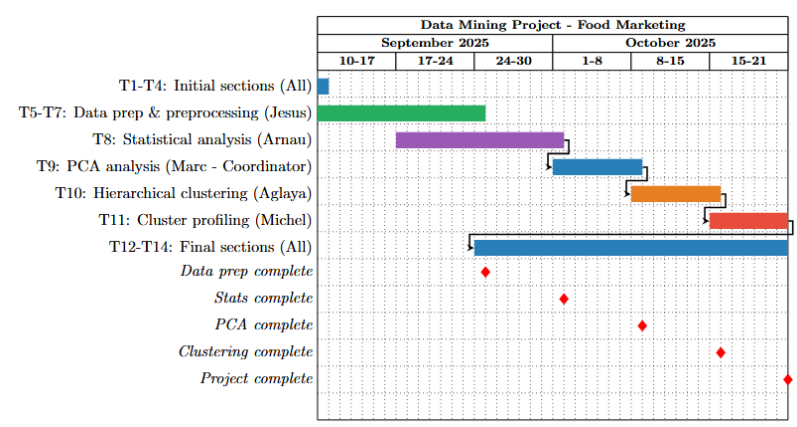
\includegraphics[width=1\linewidth]{Imatges/Gantt.pdf}
    \caption{Gantt Diagram for Tasks}
    \label{fig:gantt}
\end{figure}

% Legend
\begin{table}[H]
\centering
\begin{tabular}{cl}
\colorbox{JesusGreen}{\phantom{XX}} & Jesus Garcia Ayala - Data preparation \\[0.2cm]
\colorbox{ArnauPurple}{\phantom{XX}} & Arnau Hernández Navarro - Statistical analysis \\[0.2cm]
\colorbox{MarcBlue}{\phantom{XX}} & Marc Font I Cabarrocas - PCA analysis \& \textbf{Project Coordinator} \\[0.2cm]
\colorbox{MarcBlue!50!MichelRed!50}{\phantom{XX}} & Marc Font \& Michel Mediavilla - Hierarchical clustering \\[0.2cm]
\colorbox{MichelRed}{\phantom{XX}} & Alex Michel Mediavilla Jiménez - Cluster profiling \\[0.2cm]
\colorbox{SharedOrange}{\phantom{XX}} & All team members - Shared responsibilities \\
\end{tabular}
\end{table}


\textbf{\textcolor{secondaryblue}{Task Dependencies:}}
\begin{itemize}[leftmargin=*]
    \item T8 (Statistical analysis) depends on completion of T5-T7 (Data preprocessing)
    \item T9 (PCA analysis) depends on T8 completion 
    \item T10 (Hierarchical clustering) depends on T9 completion
    \item T11 (Cluster profiling) depends on T10 completion
    \item T12-T14 (Final sections) run in parallel but require integration of all analyses
\end{itemize}

\textbf{\textcolor{secondaryblue}{Critical Path:}} T5-T7 → T8 → T9 → T10 → T11 (Total: 48 days including overlaps)

\raggedright
\subsection{Risk-Contingency-Plan}

The following risk assessment identifies potential project challenges and establishes prevention and management strategies:

\begin{table}[H]
\centering
\tiny
\renewcommand{\arraystretch}{1.3}
\begin{tabular}{|p{2.8cm}|p{3.2cm}|p{3.8cm}|p{3.8cm}|}
\hline
\rowcolor{primaryblue!10}
\textbf{\textcolor{primaryblue}{Risk}} & \textbf{\textcolor{primaryblue}{Description}} & \textbf{\textcolor{primaryblue}{How to Prevent}} & \textbf{\textcolor{primaryblue}{How to Manage}} \\
\hline
\textbf{Team Member Unavailability} & Member becomes unavailable due to illness or personal issues & Regular communication, backup assignments for critical tasks & Redistribute work among remaining members, Jesus provides technical support to any task \\
\hline
\textbf{Data Quality Issues} & Missing values, outliers, or structural problems affecting analysis validity & Early data exploration, comprehensive preprocessing planning, document assumptions & Apply robust methods, imputation techniques, transformations. Document all decisions and impacts \\
\hline
\textbf{Technical Difficulties} & Software issues, R package conflicts, computational limitations & Test packages early, ensure compatible versions, backup environments & Use alternative tools (Python), simplify models, apply sampling techniques \\
\hline
\textbf{Analysis Method Limitations} & PCA/clustering methods unsuitable for dataset characteristics & Verify assumptions early, plan alternative methods (factor analysis, different algorithms) & Switch to non-parametric methods, apply transformations, document unsuitability reasons \\
\hline
\textbf{Time Management} & Tasks exceed estimated duration, especially complex analyses & Buffer time in schedule, early start of critical tasks, regular monitoring & Prioritize essential analyses, simplify sections, redistribute completed work \\
\hline
\textbf{Integration Challenges} & Difficulty combining PCA and clustering results coherently & Plan integration strategy early, common framework, regular team meetings & Focus on significant results, use visual methods, accept contradictions with discussion \\
\hline
\textbf{Report Quality} & Poor synthesis, unclear writing, insufficient analysis depth & Early writing assignments, multiple review cycles, detailed outlines & Peer review process, clarity focus, visual aids support \\
\hline
\textbf{Data Access Delays} & Late dataset availability or understanding & Confirm access early, request documentation in advance & Use similar public datasets, adjust scope, focus on methodological rigor \\
\hline
\end{tabular}
\caption{{Risk Assessment and Mitigation Strategies}}
\label{tab:risks}
\end{table}

\textbf{\textcolor{secondaryblue}{Task Assignment Grid:}}

\begin{table}[H]
\centering
\footnotesize
\renewcommand{\arraystretch}{1.2}
\begin{tabular}{|p{3cm}|c|c|c|c|}
\hline
\rowcolor{primaryblue!10}
\textbf{\textcolor{primaryblue}{Task}} & \textbf{\textcolor{primaryblue}{Jesus}} & \textbf{\textcolor{primaryblue}{Arnau}} & \textbf{\textcolor{primaryblue}{Marc}} & \textbf{\textcolor{primaryblue}{Michel}} \\
\hline
T1-T4: Initial sections & \textcolor{primaryblue}{\textbf{X}} & \textcolor{primaryblue}{\textbf{X}} & \textcolor{primaryblue}{\textbf{X}} & \textcolor{primaryblue}{\textbf{X}} \\
\hline
\rowcolor{lightgray!10}
T5-T7: Data prep & \textcolor{primaryblue}{\textbf{X}} & & & \\
\hline
T8: Statistical analysis & & \textcolor{primaryblue}{\textbf{X}} & & \\
\hline
\rowcolor{lightgray!10}
T9: PCA analysis & & & \textcolor{primaryblue}{\textbf{X}} & \\
\hline
T10: Hierarchical clustering & & & \textcolor{primaryblue}{\textbf{X}} & \textcolor{primaryblue}{\textbf{X}} \\
\hline
\rowcolor{lightgray!10}
T11: Profiling & & & & \textcolor{primaryblue}{\textbf{X}} \\
\hline
T12-T14: Final sections & \textcolor{primaryblue}{\textbf{X}} & \textcolor{primaryblue}{\textbf{X}} & \textcolor{primaryblue}{\textbf{X}} & \textcolor{primaryblue}{\textbf{X}} \\
\hline
\end{tabular}
\caption{\textcolor{primaryblue}{Task Assignment and Coordination Matrix}}
\label{tab:assignments}
\end{table}
